%%%%%%%%%%%%%%%%%%%%%%%%%%%%%%%%%%%%
% This is the template for submission to HPCA 2016
% The cls file is a modified from  'sig-alternate.cls'
%%%%%%%%%%%%%%%%%%%%%%%%%%%%%%%%%%%%

\documentclass{sig-alternate} 
\usepackage{mathptmx} % This is Times font

\usepackage{fancyhdr}
%\usepackage[normalem]{ulem}
\usepackage[hyphens]{url}
%\usepackage{algorithmicx,algorithm}
\usepackage{pgfplots}
\usepackage{pgfplotstable}
\usepackage{framed}
\usepackage{epsfig}
\usepackage{graphicx}

%%%%%%%%%%%---SETME-----%%%%%%%%%%%%%
\newcommand{\hpcasubmissionnumber}{NaN}
%%%%%%%%%%%%%%%%%%%%%%%%%%%%%%%%%%%%
\newcommand{\todo}[1]{\begin{framed}\textcolor{red}{TODO: #1}\end{framed}}
\fancypagestyle{firstpage}{
  \fancyhf{}
\setlength{\headheight}{50pt}
\renewcommand{\headrulewidth}{0pt}
  \fancyhead[C]{\normalsize{HPCA 2016 Submission
      \textbf{\#\hpcasubmissionnumber} \\ Confidential Draft: DO NOT DISTRIBUTE}} 
  \pagenumbering{arabic}
}  

\newtheorem{lemma}{Lemma}

%%%%%%%%%%%---SETME-----%%%%%%%%%%%%%
\title{Topologic-aware Allocation Policies for Jellyfish } 
%\author{Jose A. Pascual, Javier Navaridas, Alejandro Erickson and Ian }
%%%%%%%%%%%%%%%%%%%%%%%%%%%%%%%%%%%%

\begin{document}
\maketitle
\thispagestyle{firstpage}
\pagestyle{plain}

\begin{abstract}



\end{abstract}

\section{Introduction}
\label{introduction}

Jellyfish topology \cite{jellyfish} has been recently proposed as a high bandwidth and low latency interconnect for large scale data centers and HPC systems. In opposite to recenctly proposed server-centric datacenter networks (DCN), jellyfish is an indirect (switch-centric) network in which the servers are connected to the switches. This network is a \textit{degree-bounded} random regular graph (RRG) among the top-of-rack (ToR) switches, in which all the nodes have the same degree, are bidirectional and are connected randomly. RRGs also provide other desiderable properties for an interconnect such as low diameter, high connectivity among nodes and easy incremental expansion.

As stated in the original paper \cite{jellyfish}, routing in jellyfish is a challenge. Although jellyfish provides high connectivity among switches, classical routing policies are not able to exploit the path diversity offered. In that work the authors evaluated two well-known routing policies, shortest path (SP) and Equal-cost Multi-path (ECMP), assesing that the use of the shortest paths does not provide enough path diversity to utilize the full capacity of the network. This issue was solved using the K-Shortest Path (KSP) \cite{yen} routing policy that uses more paths at the cost of being longer. Although KSP perfoms well compared to SP and ECMP, the author in \cite{llksp} showed that jellyfish has several features that make it ineffective. In particular they stated the possibly large number of source-destinations (SD) pairs that will share the same K shortest-paths and the random number of short paths between each pair of switches. 

These works have studied jellyfish both theoretically, puting bounds to topological properties, and empirically evaluating the performance of several communication patterns. However none of them have consider the natural scenario in which this topology could be used: data centers or HPC centers where many applications run concurrently. To the best of our knowledge, there is no work devoted to evaluate the performance of such applications in this topology. The assignemnt of resources to application has been widely studied in the context of HPC. Those works clearly differenciate three stages: selection of the application to be executed, allocation of the resources to that application and mapping of the taks that compose the application to the physical servers. 

The objective of this work is the evaluation of existing allocation policies applied to jellyfish in multi-application scenarios. We will see how these policies do not perform well in jellyfish due to the random nature of this topology. Because of that, we will apply ideas taken from the HPC world and adapt them to the particularisms of jellyfish. In particular we want to define concepts of locality to jellyfish. In addition we will extend the definition of contiguity and convexity to jellyfish. These policies should improve the performance of applications executed on jellyfish. However, contiguity can severely affects system utilization. this drawback will also be studied.

The evaluation of the allocation policies has been carried out using extensive simulation with a representative mix of parallel application. Results show that tradicional and simple allocation strategies do not take advantadge of the characteristics of jellyfish. Moreover we will se how locality-aware policies can take advantadge of those properties improving the performance of applications running concurrently. In particulae locality and contiguous policies ..., We will also evaluate the drawbacks.... 

The rest of the paper is organized as follow. Section \ref{background} introduces jellyfish and communication patterns used thorough the paper. We continue in Section \ref{allocation} analyzing simple allocation policies for jellyfish introducing in Sections \cite{locality} and \cite{contiguity} the proposed policies. The results are presented and analyzed in Section \cite{results} concluding in Section \ref{conclusion} with some conlucsions and future lines of work.

\section{Background}
\label{background}

In this section we describe thoroughly the jellyfish topology and give some definitions and properties that will be used in the rest of the paper. Furthermore, we describe the four routing policies developed for jellyfish asessing the pros and cons of each one of them.

\subsection{Jellyfish topology}
\label{subsec:jellyfish}

Jellyfish is a network topology in which the switches are connected randomly. We denote jellyfish as RRG(N,k,r) where N is the number of switches, k is the number of ports of the switches and r is the number of ports used to connect to other switches.  
\begin{figure}[t]
    \centering 
    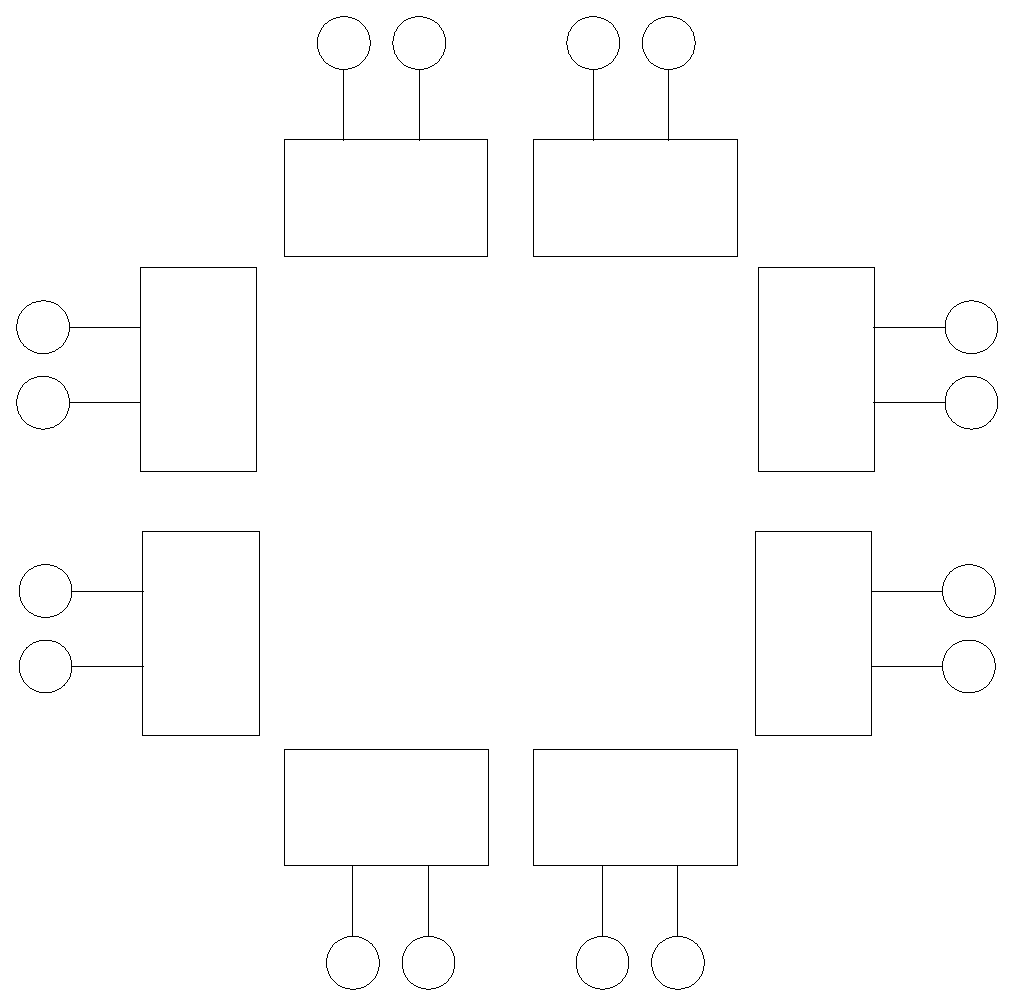
\includegraphics[width=\linewidth]{figures/jellyfish.eps}
    \caption{}
    \label{fig:jellyfish}
\end{figure}


\subsection{Routing policies}
\label{subsec:routing}

The jellyfish topology provides high path diversity between any pair of servers. This is one of the characteristic that makes this topology so appealing to execute parallel workloads. As we have seen, there exists a lot of possible paths among physical servers to carry out the communications. This is the reason why the chosing of a routing policy is so important in jellyfish in order to avoid contention in network links. There exist only four routing policies proposed and evaluated for jellyfish. Next, we will analize these policies stating the improvements of one against the others.

\begin{itemize}
    \item Shortest Path (SP):
    \item Equal-Cost Multi-Path (ECMP):
    \item K-Shortest Path:
    \item Limited Length Spread K-shortest Path (LLKSR):
\end{itemize}

\subsection{Workloads and performance metric}
\label{subsec:workloads}

\begin{itemize}
    \item Nearest neighbor:
    \item Collective:
    \item: Permutation and shift pattern:
\end{itemize}

\section{Allocation in Jellyfish}
\label{allocation}

When an application is submitted to be executed, the allocator is in charge of finding the appropiate set of resources to place it. There are many works that propose allocation policies for other topologies such as meshes, tori \cite{tori} \cite{toritree}, or fattrees \cite{toritree} \cite{trees}, but, to the best of our knowledge, not for jellyfish. Only in \cite{llksp} the authors use some simple mono-application allocation policies without taking into account how these policies behave when multiple application run concurrently. In this section we describe and analize those policies adding a new version of one of them due to random structure of jellyfish.

In order to define the allocation policies we must first assign assign a node ordering to the servers and switches that compose the network. Due to the random structure of jellyfish, we first define order the switches and then, inside each switch, we order the server consecutively.

\begin{itemize}
    \item Sequential: The tasks are assigned to the servers consecutively using the identity function.
        \begin{equation}
            \pi:T \rightarrow P\\
            \pi(t_i)=p_i
        \end{equation}
    \item Random: The tasks of the application are assigned to the servers uniformly at random.
        \begin{equation}
            \pi:T \rightarrow P\\
            \pi(t_i)=p_j where p_j is selected at random
        \end{equation}
    \item Random$^*$: This is a special version of the previouly presented policies. In this case we select a switch uniformy at random and then we map (k-r) tasks to the servers direcctly connected to it. 
        \begin{equation}
            \pi:T \rightarrow P\\
            \pi(t_i)=p_j where p_j is selected at random
        \end{equation}
\end{itemize}

\begin{lemma}

\end{lemma}
%The first two policies were evaluated in \cite{llksr} using different communication patterns mapped to the whole system. Using this configuration, the authors evaluated performance using only one application. 

%Results showed that, in average, the sequential policy performs the best. This results is expected because it maintains certain level of locality at a switch level. for some patterns such as  the random policy performs better than the sequential version.      


\begin{figure}[t]
  \begin{tikzpicture}
    \begin{axis}[width=\linewidth,
    %height=5cm,
    %    scale only axis,
    %    axis y line*=left,
    %    ytick={0,1,2,3,4,5,6,7,8,9,10,11,12,13,14,15,16,17,18,19},
    ylabel={Completion time (s)},
    xtick={0,1,2,3,4,5},
    xticklabels={
        1,
      2,
      3,
      4,
      5,
      6
  },
    x tick label style={rotate=90,anchor=east},
    ybar=0pt,
    bar width=6,
    unbounded coords=jump,
    %    grid=major,
    legend entries={
        1,      
      2,
      3,
        4
    },
    legend style={font=\footnotesize},
    legend pos=north west,
    %    mark size=4
    ]
    % \addplot+[only marks,mark=asterisk,error bars/.cd,y dir=both,y explicit]   
    % table [x=x,y=y,y error expr= \thisrow{sigma}*1.96] {
    \addplot+[
    ]
    table[
        meta=network,
    x expr=\coordindex,
    y=DR,
    %y expr=100.0*(\thisrow{mean_dr_list}-\thisrow{mean_bfs})/\thisrow{mean_dr_list},
]
    {plots/data/all2one.dat};
    \addplot+[
        % \iferrorbars
        % error bars/.cd,
        % y dir=both,
        % y explicit
        % \fi
    ]
    table[
        meta=network,
    x expr=\coordindex,
    y =GPE,
    % \iferrorbars
    % y error expr=\thisrow{std_savings_ex_list}/100
    % \fi
]
    {plots/data/all2one.dat};
    \addplot+[
        % \iferrorbars
        % error bars/.cd,
        % y dir=both,
        % y explicit
        % \fi
    ]
    table[
        meta=network,
    x expr=\coordindex,
    y =GPI,
    % \iferrorbars
    % y error expr=\thisrow{std_savings_int_list}/100
    % \fi
]
    {plots/data/all2one.dat};
    \addplot+[
        % \iferrorbars
        % error bars/.cd,
        % y dir=both,
        % y explicit
        % \fi
    ]
    table[
        meta=network,
    x expr=\coordindex,
    y = GP0,
    %discard if={k}{2},
    % \iferrorbars
    % y error expr=\thisrow{std_savings_ti_list}/100
    % \fi
]
    {plots/data/all2one.dat};
\end{axis}
     
  \end{tikzpicture}
  \caption{Completion time in second employed to process three traffic patterns comparing.}
\label{fig:plot-dynamic}
\end{figure}


\section{Link utilization in jellyfish}
\label{linkutilization}



\section{Locality and Contiguity in Jellyfish}
\label{locality}

\section{Experimental Set-up}
\label{experimental}

\subsection{Simulation environment}
\label{subsec:simulation}


\subsection{Communication patterns}
\label{subsec:communication}

\subsection{Performance metrics}
\label{subsec:performance}


\section{Analysis of the Results}
\label{analysis}

\section{Conclusiosn ans Future Work}
\label{conclusions}

%%%%%%% -- PAPER CONTENT ENDS -- %%%%%%%%

%%%%%%%%% -- BIB STYLE AND FILE -- %%%%%%%%
\bibliographystyle{ieeetr}
\bibliography{hpca16}
%%%%%%%%%%%%%%%%%%%%%%%%%%%%%%%%%%%%

\end{document}
